\documentclass{beamer}

%\usepackage[latin2]{inputenc}
%\usepackage[T1]{fontenc}
\usepackage{amsmath,amssymb} % AMS matematikai és fontcsomag
\usepackage{amsthm}          % tételszerű környezetek
\usepackage{graphicx}        % képek beillesztéséhez
\usepackage{geometry}        % méretek állítása
\usepackage{subcaption} 	 % subfigure
\usetheme{Warsaw}
\useoutertheme{miniframes} % Alternatively: miniframes, infolines, split
\useinnertheme{circles}
\usecolortheme{crane}

\newtheorem{thm}{Theorem}
\newtheorem{defi}[thm]{Definition}
\newtheorem{lem}[thm]{Lemma}
\newtheorem{cor}[thm]{Corollary}
\newtheorem{prop}[thm]{Proposition}
\newtheorem{rem}[thm]{Remark}

\def\IR{\mathbb{R}}
\def\IT{\mathbb{T}}
\def\IN{\mathbb{N}}
\def\IZ{\mathbb{Z}}
\def\SS{\mathbb{S}}

\usepackage{worldflags}
\flagsdefault[width=4pt, length=6pt, framewidth=0.1mm]

\title{Changes in the connection networks of MEPs}
\author[Marits Márton, Bernát Ádám]{Marits Márton, Bernát Ádám}
\institute[BME]
{ Budapesti Műszaki és Gazdaságtudományi Egyetem \\
					\textbf{Project Laboratory}								}
\date{2023}

\begin{document}

\begin{frame}
\titlepage
\end{frame}

\begin{frame}
\frametitle{Introduction}
By its plastic nature, human connections change over time, especially when outside effects take place. However, in the case of policy makers, such changes will sooner or later have consequences to our life (As we live in the EU.)
\end{frame}


\begin{frame}
\frametitle{Motivation}

Understanding the network of MEPs might give us a better understanding of the following:

\bigskip

\begin{itemize}
	\pause \item How smaller networks inbetween MEPs look like, their size and their quantity.
	
	\pause \item \textbf{Identifying key decision and policy makers.}
	
	\pause \item \textbf{How events and occurrences shape the form and topology of the network.}

\end{itemize}

\pause All of these are helpful in understanding the processes regarding proposals and how they evolve into enacted laws.

\end{frame}



\begin{frame}
\frametitle{Our Topic(s)}

\bigskip

\begin{itemize}
	\pause \item \textbf{Our main focus was on the effects of COVID-19 and how it shaped the network of MEPs.}
	
	\pause \item A more recent topic of interest might be the Russian-Ukrainian conflict and how it altered connections within the European Parliament.
	
	\pause \item For now, we focused on gathering information on \textbf{the whole dataset at once}, and we will focus on the changes over time in future research

\end{itemize}
\end{frame}



\begin{frame}
\frametitle{Our analysis}

\begin{columns}

\column{5cm}

We acquired data regarding amendments, for each amendment we know which MEP proposed the amendment, what kind of document it is, etc..
\bigskip

\pause Basically, we got a bipartite graph with node groups:
\begin{itemize}
	\item MEPs
	\item Documents
\end{itemize}
\bigskip

\pause Edges $\iff$ MEP made amendment to document

\pause \column{5cm}
\begin{center}
\small{A bipartite graph:}
\bigskip
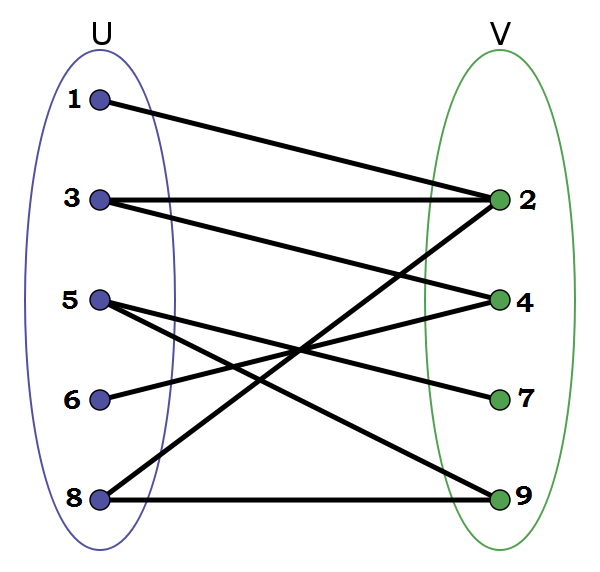
\includegraphics[height=3.2cm]{BipartiteGraph.png}
\end{center} 

\end{columns}
\end{frame}



\begin{frame}
\frametitle{Projection}

We then created a projection of this bipartite graph:

\begin{itemize}
	\pause \item Nodes: the nodes of MEPs
	\pause \item Edges: 2 MEPs are connected if they amended the same document	
\end{itemize}

\pause We have also considered and implemented weighted projection. We used the so called: "Collaboration weighted projection"(where we reward secluded document matching and punish popular document matching)

\end{frame}

\begin{frame}
	\frametitle{Analysis of activity by country}
	We are interested in analyzing how many amendments were contributed by each country's MEPs.
	
	\vspace{0.3cm}
	
	\pause {\tiny \begin{tabular}{| l | r |}
		\hline
		Country & Contributions  \\
		\hline
		\worldflag{DE} Germany & 5539 \\
		\worldflag{FR} France & 4242 \\
		\worldflag{ES} Spain & 3853 \\
		\worldflag{IT} Italy & 3550 \\
		\worldflag{PL} Poland & 2531 \\
		\multicolumn{1}{|c|}{\vdots} & \multicolumn{1}{|c|}{\vdots} \\
		\worldflag{LT} Lithuania & 541 \\
		\worldflag{CY} Cyprus & 502 \\
		\worldflag{LV} Latvia & 426 \\
		\worldflag{EE} Estonia & 423 \\
		\worldflag{GB} United Kingdom & 268 \\
		\hline
	\end{tabular}}

	\vspace{0.3cm}

	\pause As one would expect, largest countries on top, small countries on the bottom.
	
	\pause The UK is an outlier because of Brexit, as one would expect.
	
	\pause (They left the European Parliament in January 2020)
	
\end{frame}

\begin{frame}
	\frametitle{Analysis of activity by country}
	Okay, so what if we normalize for population?
	
	\vspace{0.3cm}
	
	\pause {\tiny \begin{tabular}{| l | r |}
			\hline
			Country & Contributions per million people  \\
			\hline
			\worldflag{MT} Malta & 1181.76 \\
			\worldflag{LU} Luxembourg & 965.30 \\
			\worldflag{CY} Cyprus & 546.78 \\
			\worldflag{SI} Slovenia & 360.67 \\
			\worldflag{EE} Estonia & 317.61 \\
			\multicolumn{1}{|c|}{\vdots} & \multicolumn{1}{|c|}{\vdots} \\
			\worldflag{DE} Germany & 66.54 \\
			\worldflag{PL} Poland & 66.54 \\
			\worldflag{FR} France & 65.01 \\
			\worldflag{IT} Italy & 60.32 \\
			\worldflag{GB} United Kingdom & 4.00 \\
			\hline
	\end{tabular}}

	\vspace{0.3cm}
	
	\pause Here we see the smaller countries dominate the scene
	
	\pause This is because EP seats are not distributed according to population
	
	\pause More seats are given to smaller countries to boost their influence in the EP
	
\end{frame}

\begin{frame}
	\frametitle{Analysis of activity by country}
	So we should normalize for number of MEPs
	
	\vspace{0.3cm}
	
	\pause {\tiny \begin{tabular}{| l | r |}
			\hline
			Country & Contributions per MEP  \\
			\hline
			\worldflag{LU} Luxembourg & 103.83 \\
			\worldflag{MT} Malta & 102.33 \\
			\worldflag{SI} Slovenia & 95.00 \\
			\worldflag{SK} Slovakia & 92.38 \\
			\worldflag{CY} Cyprus & 83.67 \\
			\multicolumn{1}{|c|}{\vdots} & \multicolumn{1}{|c|}{\vdots} \\
			\worldflag{PL} Poland & 49.63 \\
			\worldflag{LT} Lithuania & 49.18 \\
			\worldflag{IT} Italy & 48.63 \\
			\worldflag{CZ} Czechia & 48.57 \\
			\worldflag{GB} United Kingdom & 3.67 \\
			\hline
	\end{tabular}}

	\vspace{0.3cm}
	
	\pause The smaller countries do more, even in this chart
	
	\pause So the \textbf{MEPs of smaller countries contribute more} on average
	
\end{frame}

\begin{frame}
	\frametitle{Analysis of activity by EP Group}
	Which EP Groups were the most active?
	
	\pause EP groups are coalitions of parties from different countries
	
	\pause The current EP groups are the following:
	
	\vspace{0.3cm}
	
	\pause {\tiny \begin{tabular}{| l | l | r |}
			\hline
			EP Group & Ideology & MEPs (pre-Brexit)  \\
			\hline
			European People's Party (EPP) & center-right, conservative & 176 (182) \\
			Socialists and Democrats (S\&D) & social democrat, progressive & 144 (154) \\
			Renew Europe (RE) & liberal, pro-Europe & 101 (108) \\
			Greens-European Free Alliance (Greens/EFA) & green, regionalist, pro-Europe & 73 (72) \\
			European Conservatives and Reformists (ECR) & conservative & 66 (62) \\
			Identity and Democracy (ID) & nationalist, euroskeptic & 62 (73) \\
			European United Left/Nordic Green Left (GUE-NGL) & socialist, euroskeptic & 37 (41) \\
			Non-inscrits (NI) & various & 46 (57) \\
			\hline
			
			\hline
	\end{tabular}}
	
	\vspace{0.3cm}
	
	\pause ``Non-inscrits" is a French term for ``non-aligned"
	
\end{frame}

\begin{frame}
	\frametitle{Analysis of activity by EP Group}
	Which EP Groups were the most active?
	
	\pause We gathered the following data on activity by EP Group:
	
	\vspace{0.3cm}
	
	\pause {\tiny \begin{tabular}{| l | l | r |}
			\hline
			EP Group & \#MEPs & Contribs/MEP\\
			\hline
			RE & 108 & 83.29 \\
			S\&D & 154 & 75.79 \\
			EPP & 182 & 73.54 \\
			GUE/NGL & 41 & 44.29 \\
			ECR & 62 & 34.16 \\
			Greens/EFA & 74 & 30.92 \\
			ID & 73 & 28.63 \\
			NI & 54 & 11.37 \\
			\hline
	\end{tabular}}
	
	\vspace{0.3cm}
	
	\pause We see that MEPs from the \textbf{left-wing and liberal parties} contribute the most amendments.
	
	\pause There is also a tendency for larger EP groups to contribute more.
	
\end{frame}

\begin{frame}
	\frametitle{Centrality of MEPs}
	Which MEPs are the most central?
	
	\pause We analyze the `degree centrality' of each MEP in the social network graph
	
	\pause How many different co-contributors does each MEP have?
	
	\vspace{0.3cm}
	
	\pause {\tiny \begin{tabular}{| l | l | r |}
			\hline
			MEP & EP Group & Degree centrality  \\
			\hline
			\worldflag{BE} Hilde Vautmans & RE & 183 \\
			\worldflag{DK} Karen Melchior & RE & 173 \\
			\worldflag{LU} Marc Angel & S\&D & 169 \\
			\worldflag{BE} Olivier Chastel & RE & 167 \\
			\worldflag{PL} Łukasz Kohut & S\&D & 166 \\
			\worldflag{SK} Michal Šimečka & RE & 160 \\
			\worldflag{SK} Michal Wiezik & EPP & 152 \\
			\worldflag{RO} Ramona Strugariu & RE & 151 \\
			\worldflag{LT} Petras Auštrevičius & RE & 151 \\
			\worldflag{IE} Maria Walsh & EPP & 146 \\
			\hline
	\end{tabular}}
	
	\vspace{0.3cm}
	
	\pause The most central MEPs come from \textbf{smaller and mid-sized countries}
	
	\pause They mostly come from the more left-wing EP Groups such as RE or S\&D.
	
\end{frame}


\begin{frame}
\frametitle{Behavior of central nodes}
\begin{columns}
\column{5cm}
Betwenness centrality \\
2020 as basis:
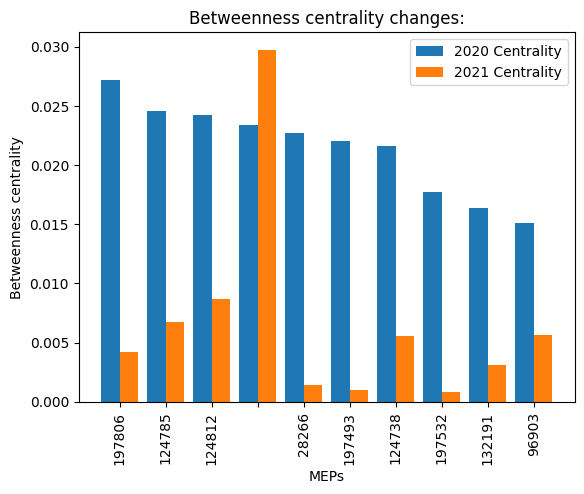
\includegraphics[height=4cm]{Betweeness_2020asBasis.png}

\pause \column{5cm}
Eigenvector centrality \\
2021 as basis:
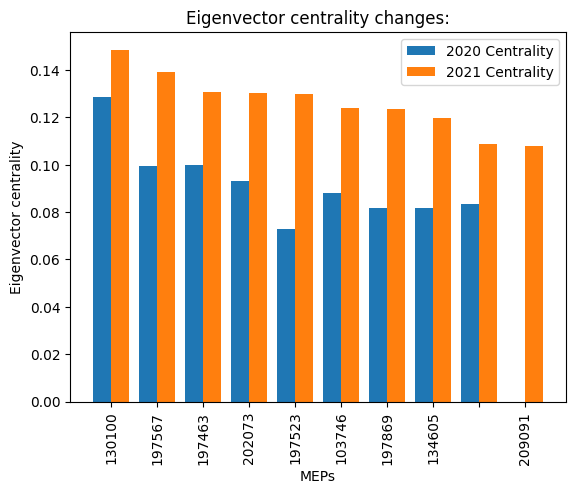
\includegraphics[height=4cm]{Eigenvector_2021asBasis.png}

\end{columns}
\end{frame}


\begin{frame}
	\frametitle{Projection}
	Some visualizations of the MEP social network graph (there were also some 0 degree nodes):
	\pause
	\begin{center}
		\includegraphics[height=5.6cm]{plain_picture.png}
	\end{center} 
	\pause 
	{\tiny The Smaller interval ones look similar, however they aren't necessarily connected like this one}
	
	
\end{frame}

\begin{frame}
	\frametitle{Projection}
	Color coding the nodes (according to EP groups):
	\pause
	\begin{center}
		\includegraphics[height=6.2cm]{PM_group_Colors.png}
	\end{center} 
	
\end{frame}




\begin{frame}
\frametitle{What's next?}

We require additional data for multiple reasons:

\begin{itemize}

	\item Cutting at more relevant dates, for finer distiction.
	
\bigskip

Further consideration might be fruitful, namely, the further useage of weighted projection. (Some machine learning opportunity)

\end{itemize}
\end{frame}



\begin{frame}
\begin{center}
\Large{\textbf{Thank you for your attention!}}
\end{center}
\end{frame}


\end{document}
